%&latex
\documentclass{scrreprt}

%+Make Index
\usepackage{makeidx}
\makeindex
%-Make Index
\usepackage{graphicx}

\begin{document}

%+Title
\title{\Huge\bf Notes on Limbo21}
\author{Xiyue}
\date{\today}
\maketitle
%-Title


\chapter{Overview}
Limbo represents a MPCitH-based proof system and its NIZK variant. It is improved based on Ligero. The main improvement lies in the flexibility of good soundness error and proof size. They also propose two parralel methods for multiplication check over the sharing schemes. 

\section{Ligero}

\subsection {Packed Secret Sharing}
Pick a random $t+l$-degree polynomial $p$ such that $p(0), p(-1),�, p(-l)$ are secrets. Distribute $p(1),\cdots, p(n)$, $t+l$ shares don't reveal secret.
Therefore, a reconstruction of polynomials take $T+L$ elements, but can only preserver privacy up to $T$ parties.

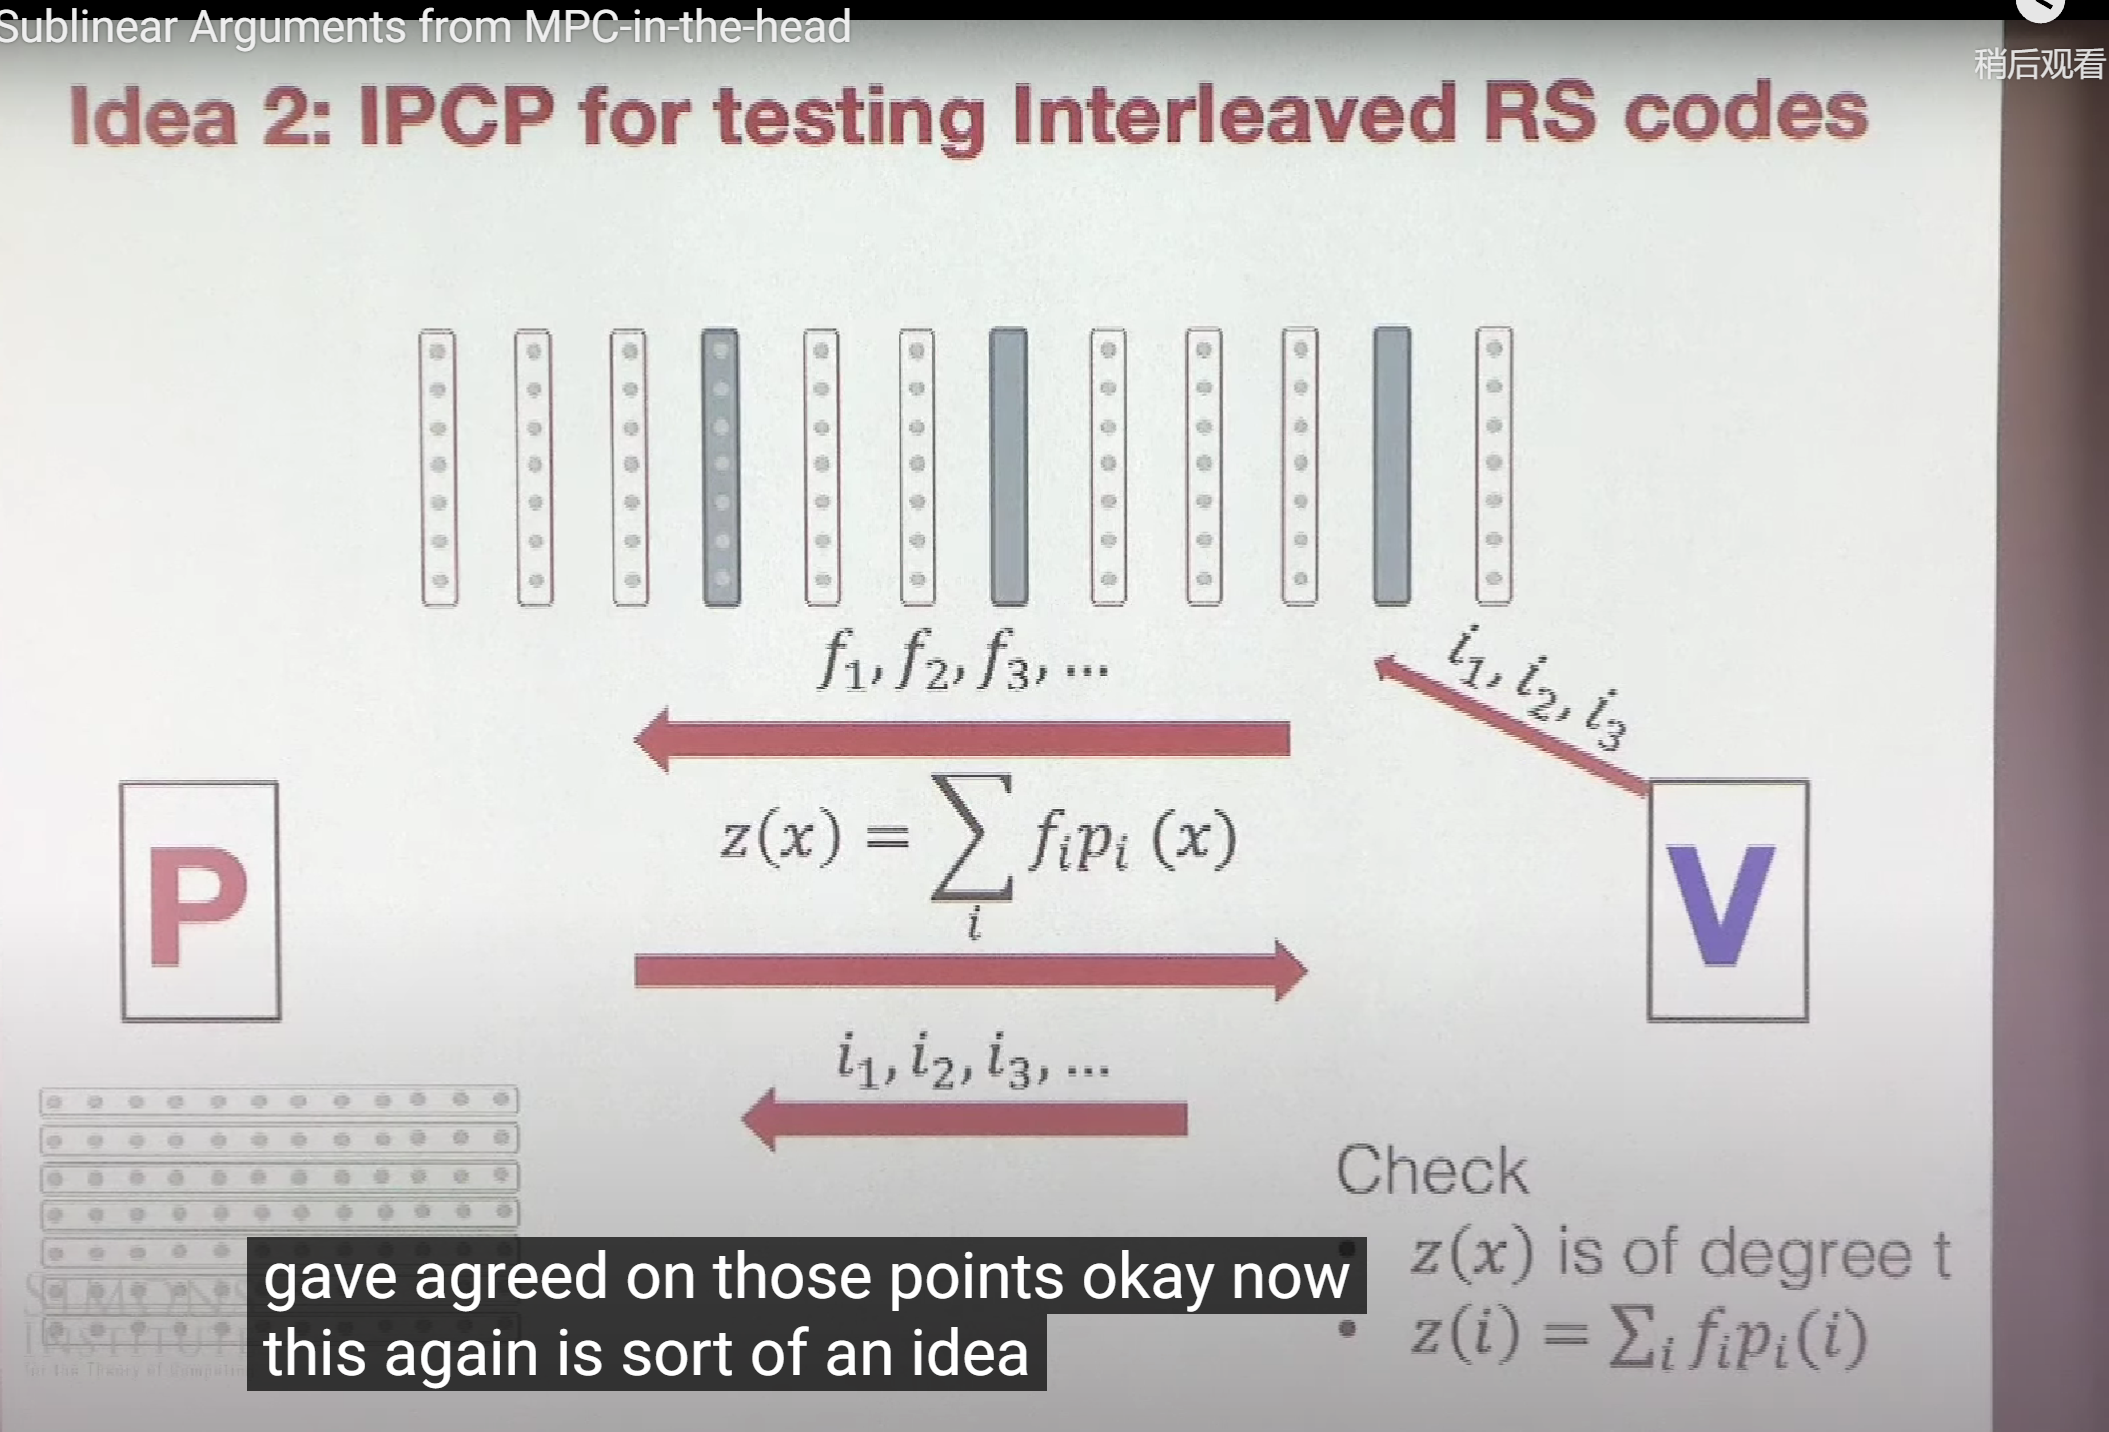
\includegraphics{image001.png}
(should be degree of t+L).

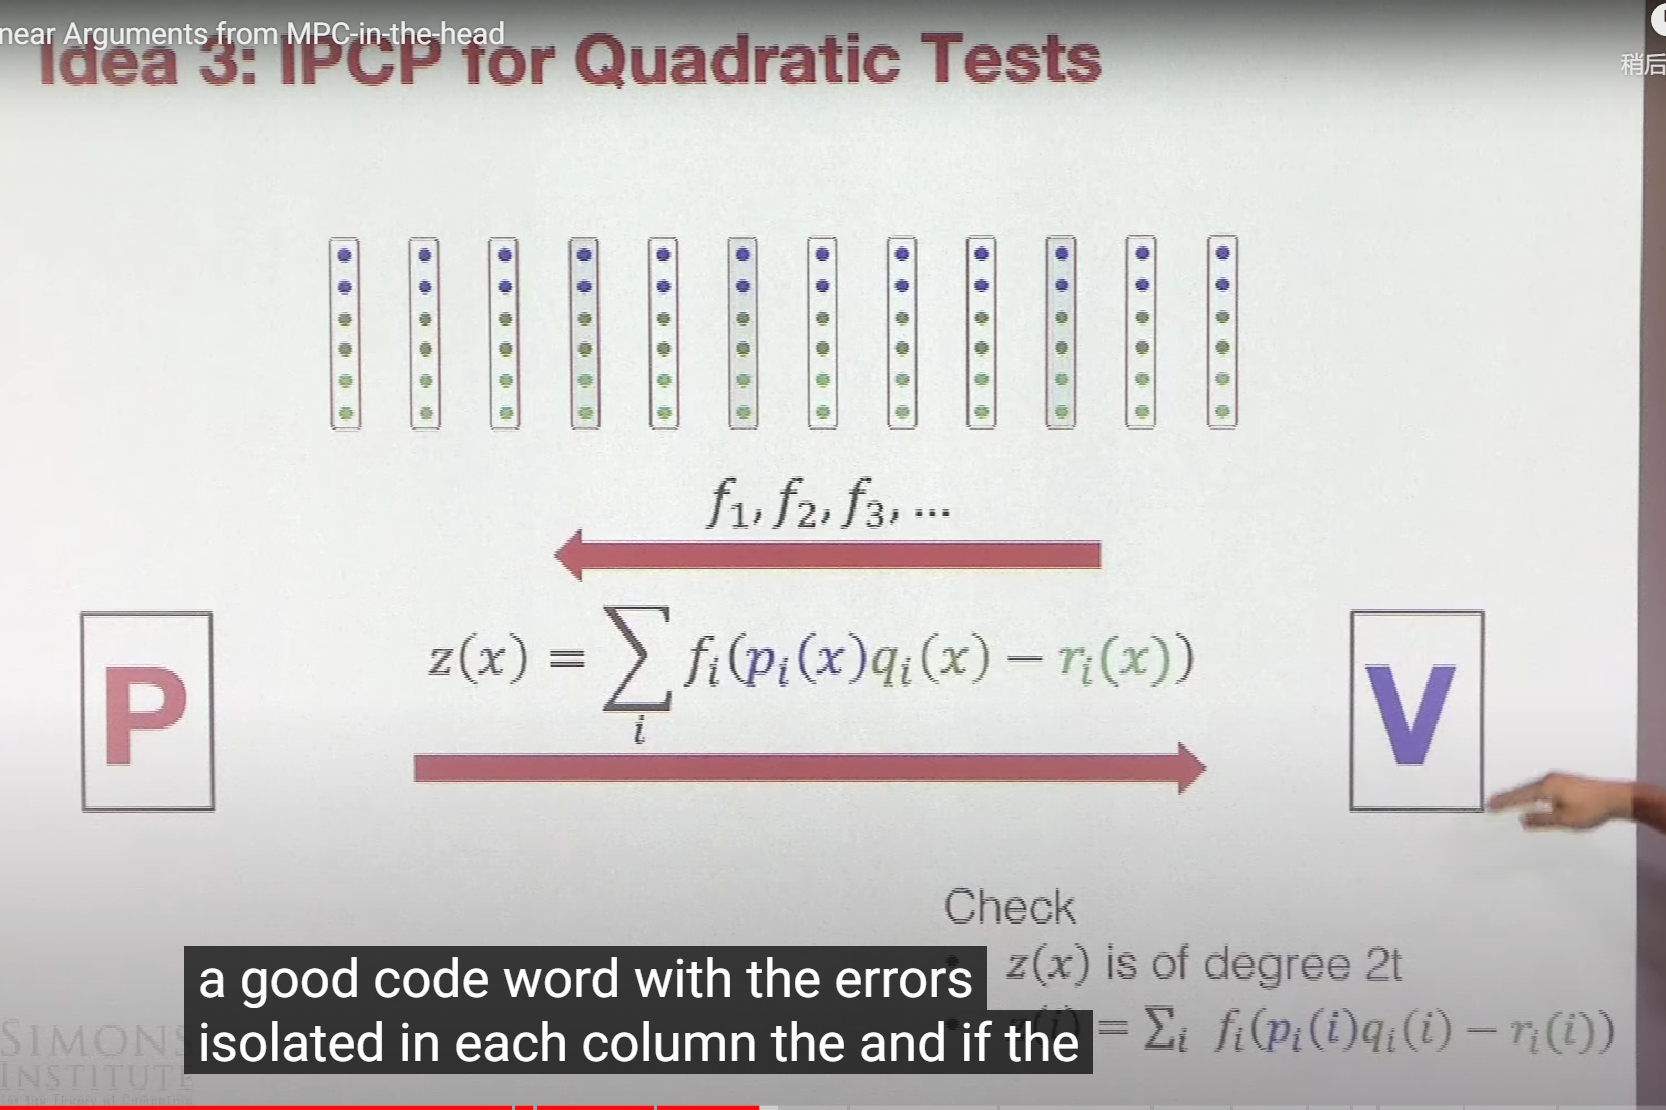
\includegraphics{image002.png}

QUESTION 1: 28:00 why cancel out the red and green ones?
QUES 2: 30:00 why must it be in order and repeat it more than twice?
and why must it check one row is the permutation of another?

\subsection {Black box computation}
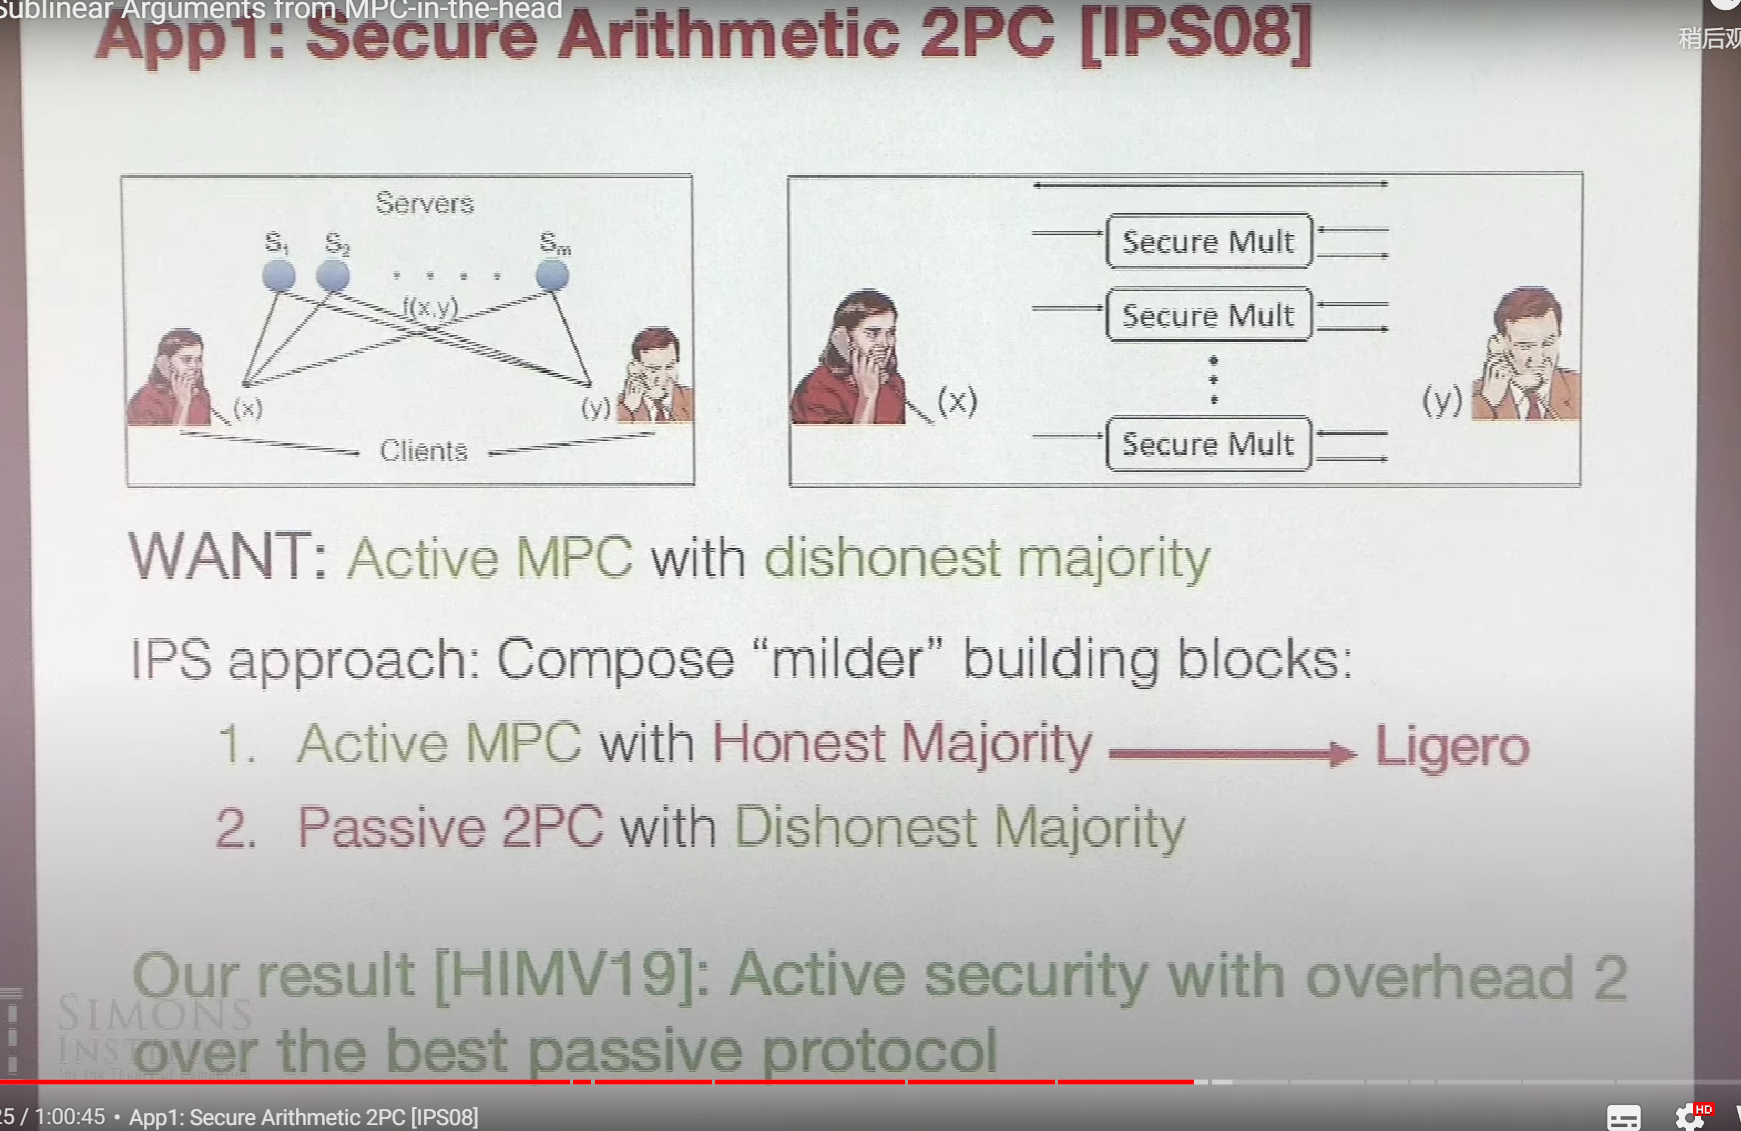
\includegraphics{image003.png}
Application with Ishai's secure computation is very interesting: combines the milder building blocks for semi-honest and malicious models. Hence reaching an overhead of twice an active security(the previous concrete approaches only is linear in the security parameters or e.g. in larger fields ).

Example: turning OLE to active implementation
Scenarios like OLE where parallel executions are engaged and .
Alice encodes and does the secret sharing of her input and sends it to the server, the server computes and sends it to Bob. So two active security guarantees: 1) the majority of the servers? did the computation correctly 2) everyone encodes the information correctly. (Corresponding to Ligero where most of the openings of the values are fine, errors are only concentrated in a few columns and the relationships between the values are preserved perfectly.)


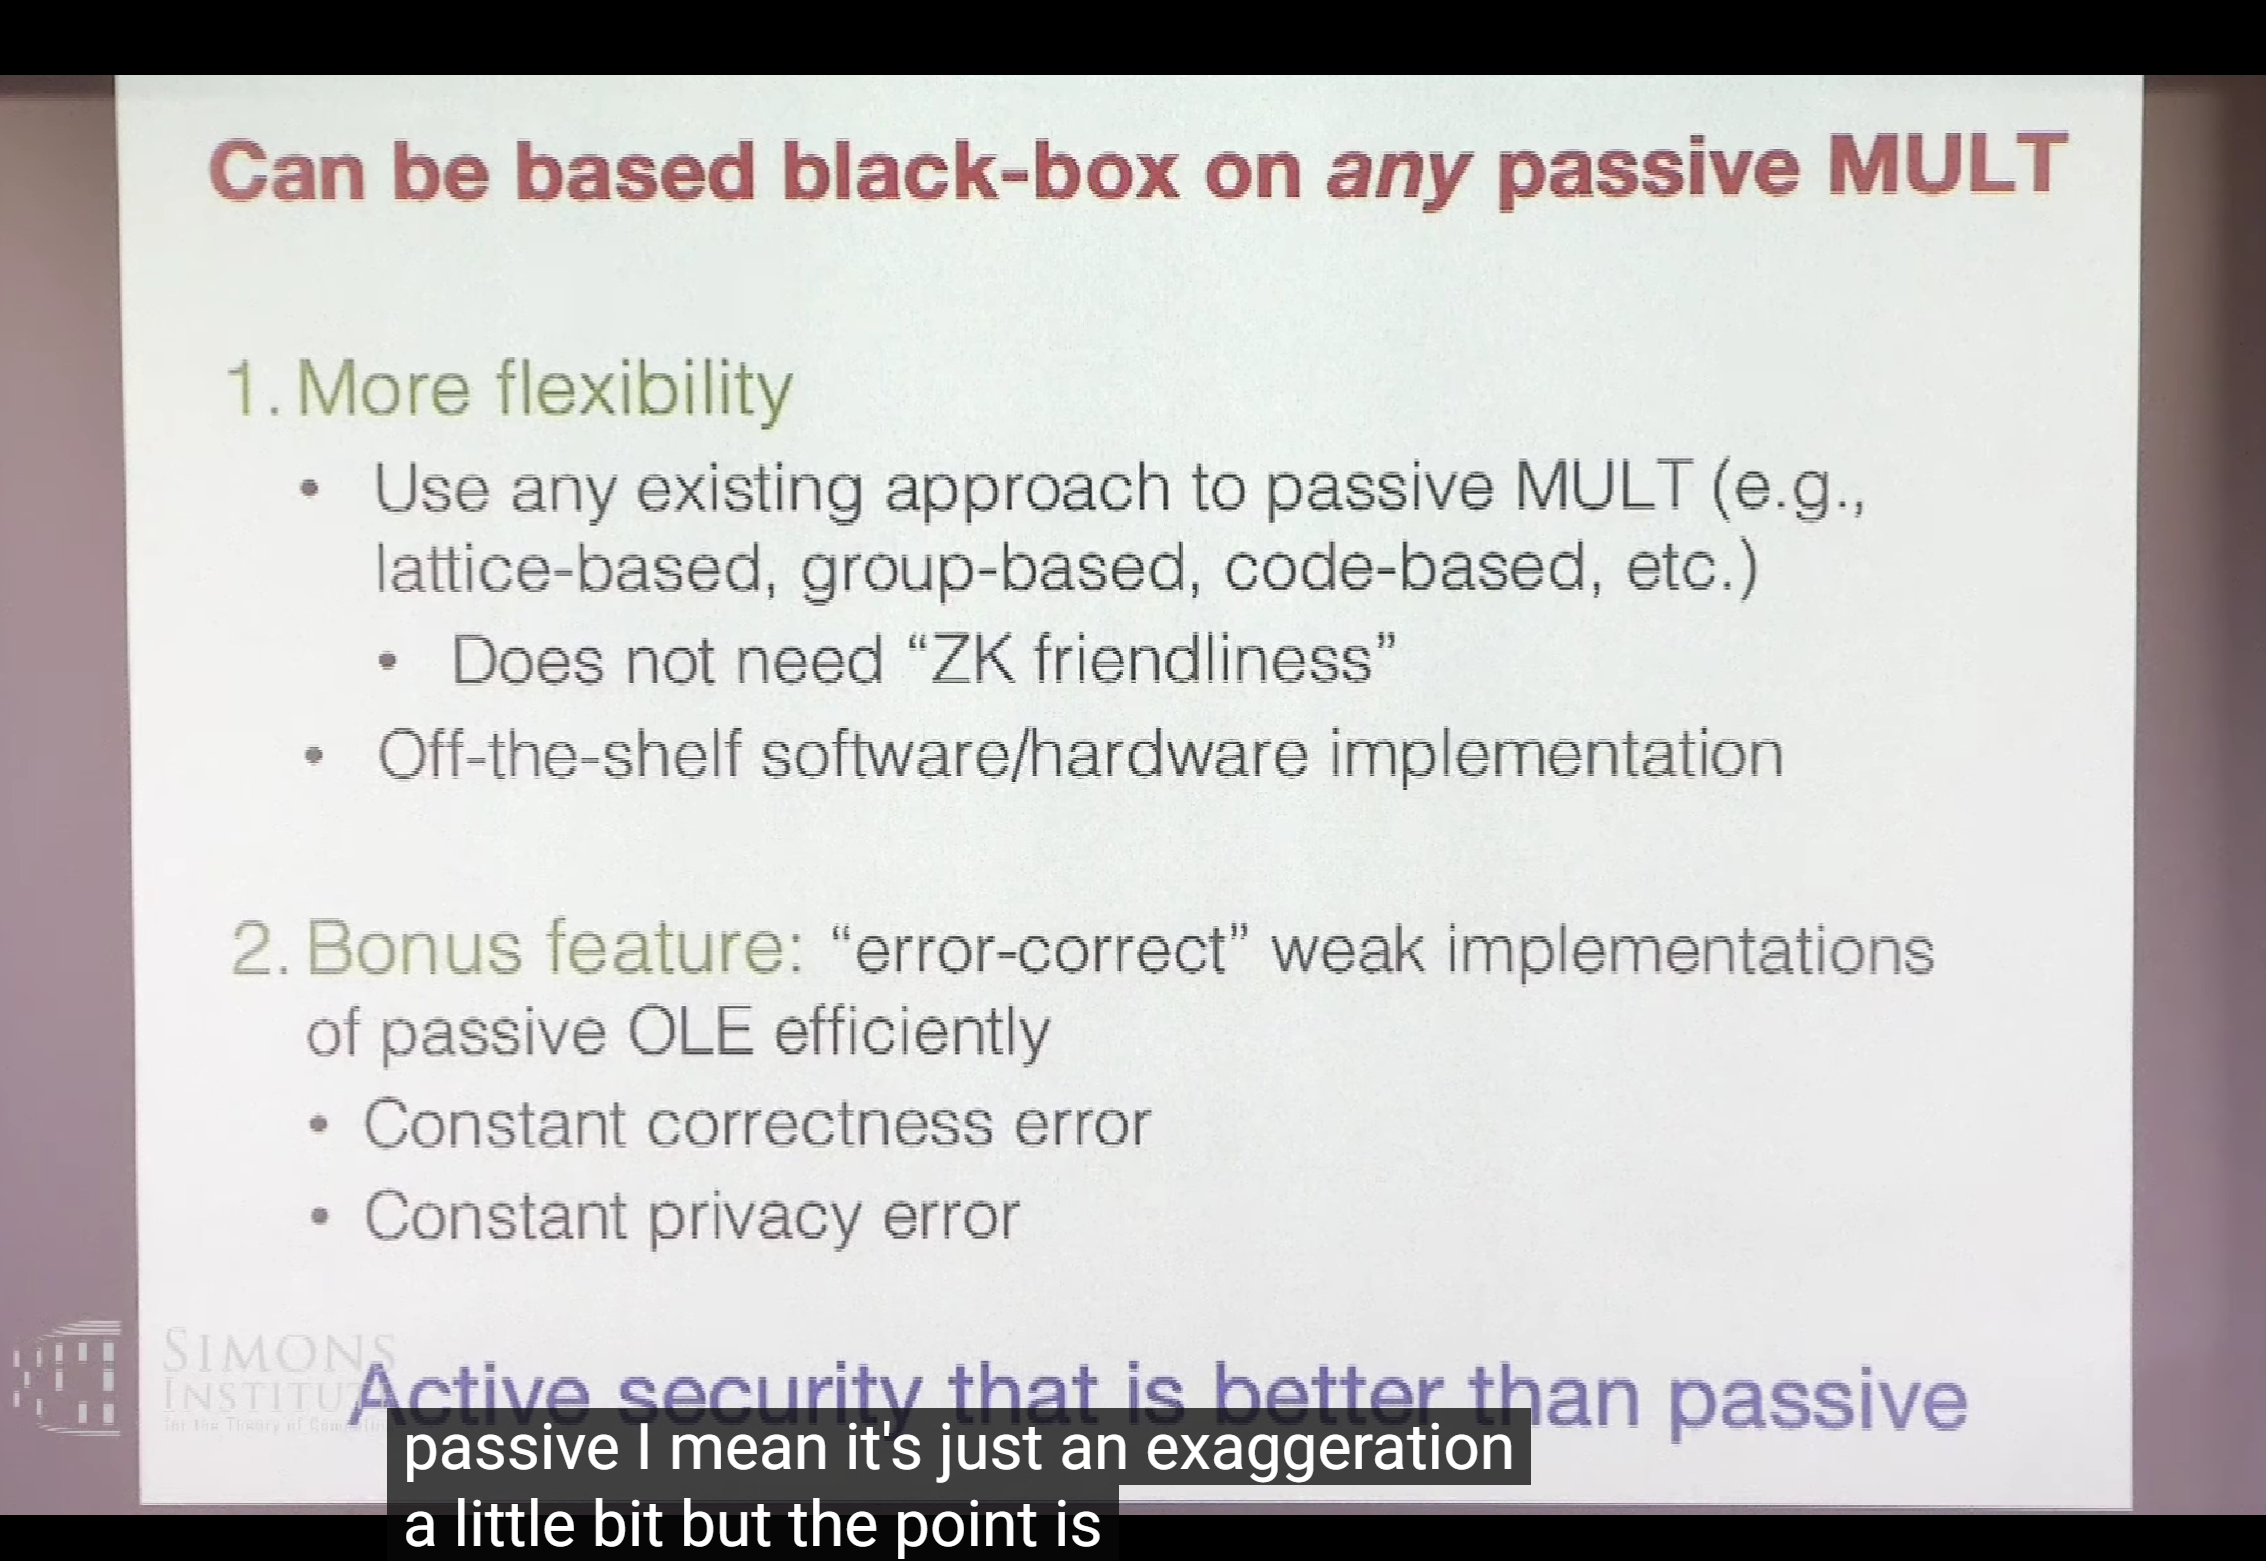
\includegraphics{image004.png}

\subsection {non-Black box computation}
For example in the certified oblivious transfer, they make a NIZK variant of Ligero to 1)only contain one garbled circuits and other features brought by NIZK 2) the computation contains non-black box cryptographical computation like verifying the computation of AES.

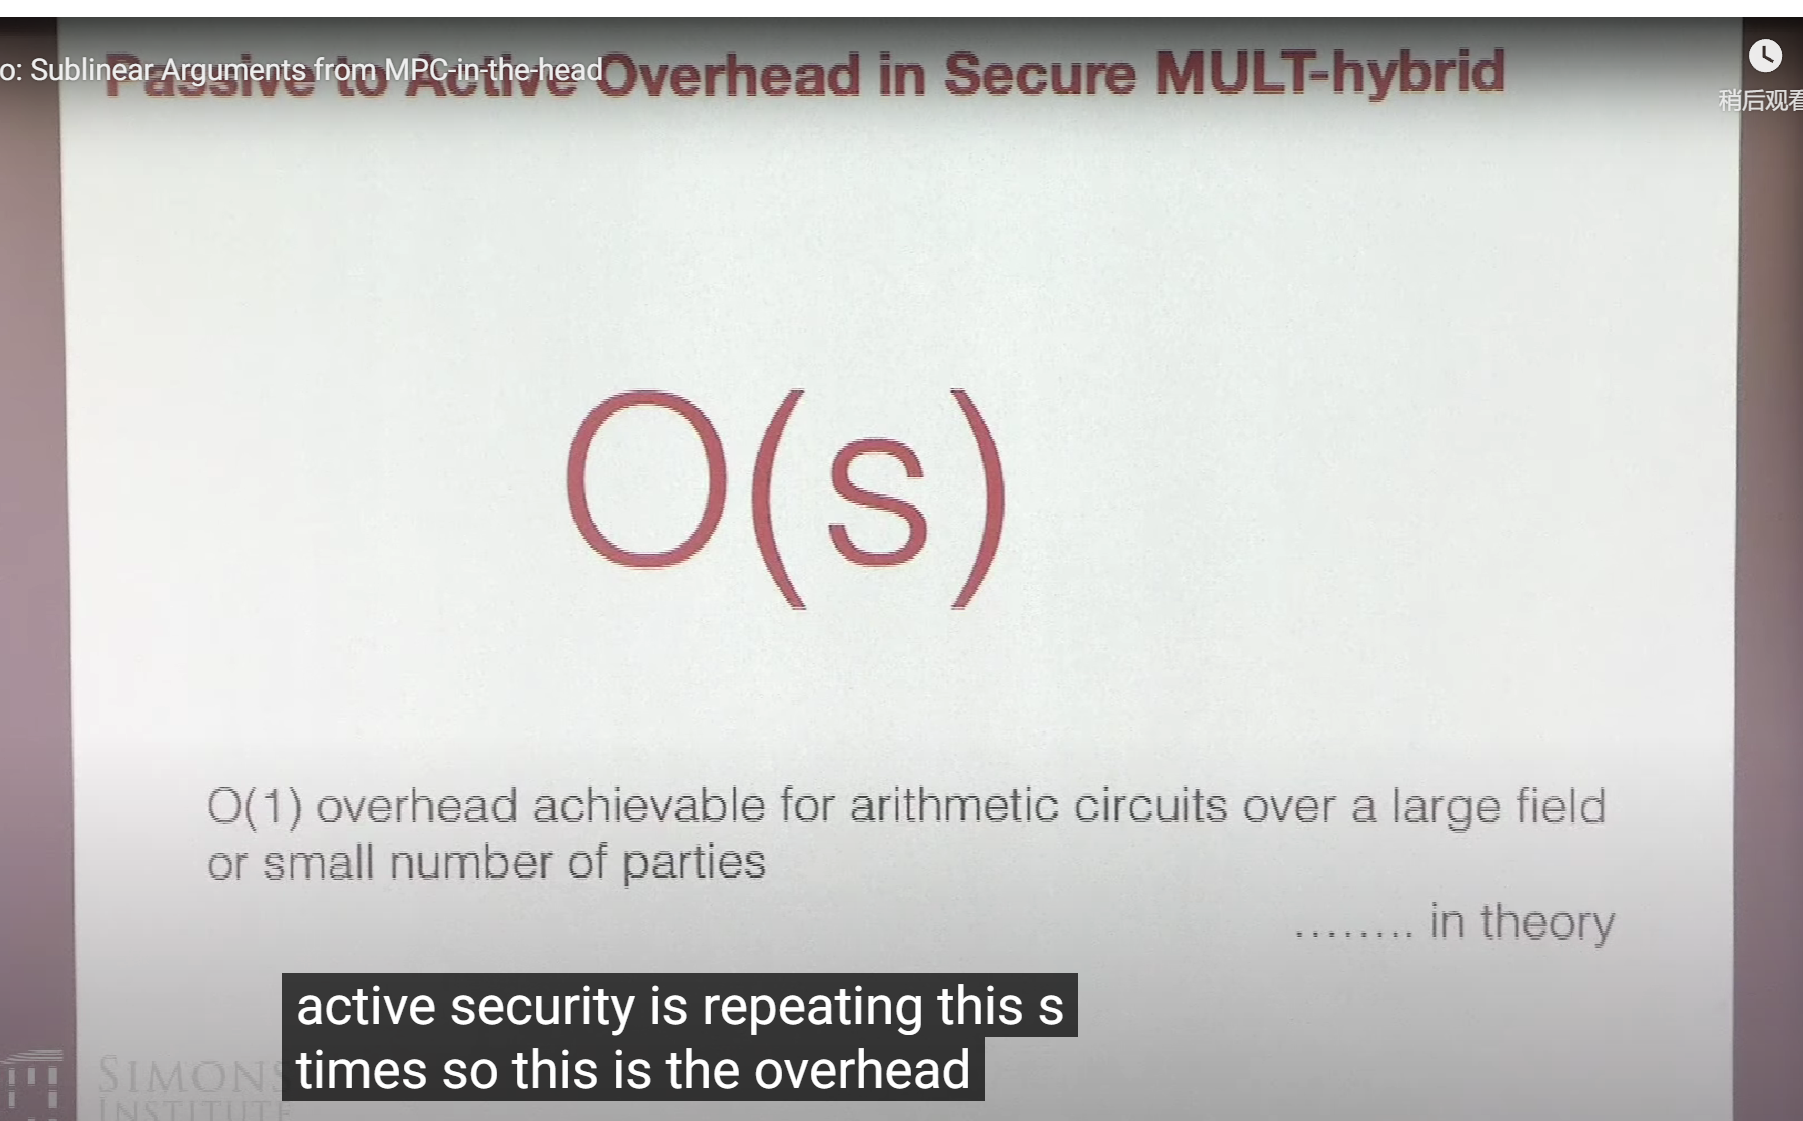
\includegraphics{image005.png}

QUES 3: 47:55 why is O(1) communication overhead achievable? (now O(1) computation overhead is still an open problem.)

Open questions:1)apart from MPC based , will other IOPs also be more efficient?s

\section{Improvement}



\section{General Construction of MPCitH based IOP}

\subsubection{Framework}

1. the servers receive the input message m1 from $P_S$ and locally compute.

2. For each phase $j \in [2, \rho- 1]$: (a) The servers call RandomCoin and obtain a public random string $R_{j-1}$ and a single message $m_j$ from PS.
 (b) The servers use the random string (and $m_j$) to continue their local computation. 

3.  the servers obtain a public random string $R$ and each sends a single message to the receiver client $P_R$.

\subsubsection{Soundness}

Why is it crucial to combine the privacy and robustness?

optimization techinques: $\tau$-parallel executions


\subsection{Multiplication Check}

\subsubsection{first}
\subsubsection{second}

\subsection{NIZK variant}


\section{Performance}

\subsection{Code}
 
\subsubsection{GF2E}

data structure: msb(the 65th-bit),modulus(characteristic p), byte\_size(data's byte size), data(the 64-bit unsigned data for polynomial), reduce(method for reducing the data into G2\_{16,64,...},did not implement any arbitrary k for $G2^k$). This is an element in GF2E.

construction: build\_from\_roots(build from ), from\_bytes(to\_bytes) 

basic operations: inverse, multiplication, addition(subtraction, because it is GF2 data structure.)

calculations: lift, first\_N\_elements, precompute\_lagrange\_polynomials, interpolate\_with\_precomputation, horner eval, compute\_powers, dot\_product, init\_extension\_field?




%+Bibliography
\begin{thebibliography}{99}
\bibitem{Label1} ...
\bibitem{Label2} ...
\end{thebibliography}
%-Bibliography

%+MakeIndex
\printindex
%-MakeIndex


\end{document}


